\documentclass[border=10pt]{standalone}
\usepackage[svgnames]{xcolor}
\usepackage{amsmath}
\usepackage{pgfplots}
\pgfplotsset{compat=newest}
\usepackage[sfdefault]{FiraSans}
\usepackage{FiraMono}
\renewcommand*\familydefault{\sfdefault}
\begin{document}
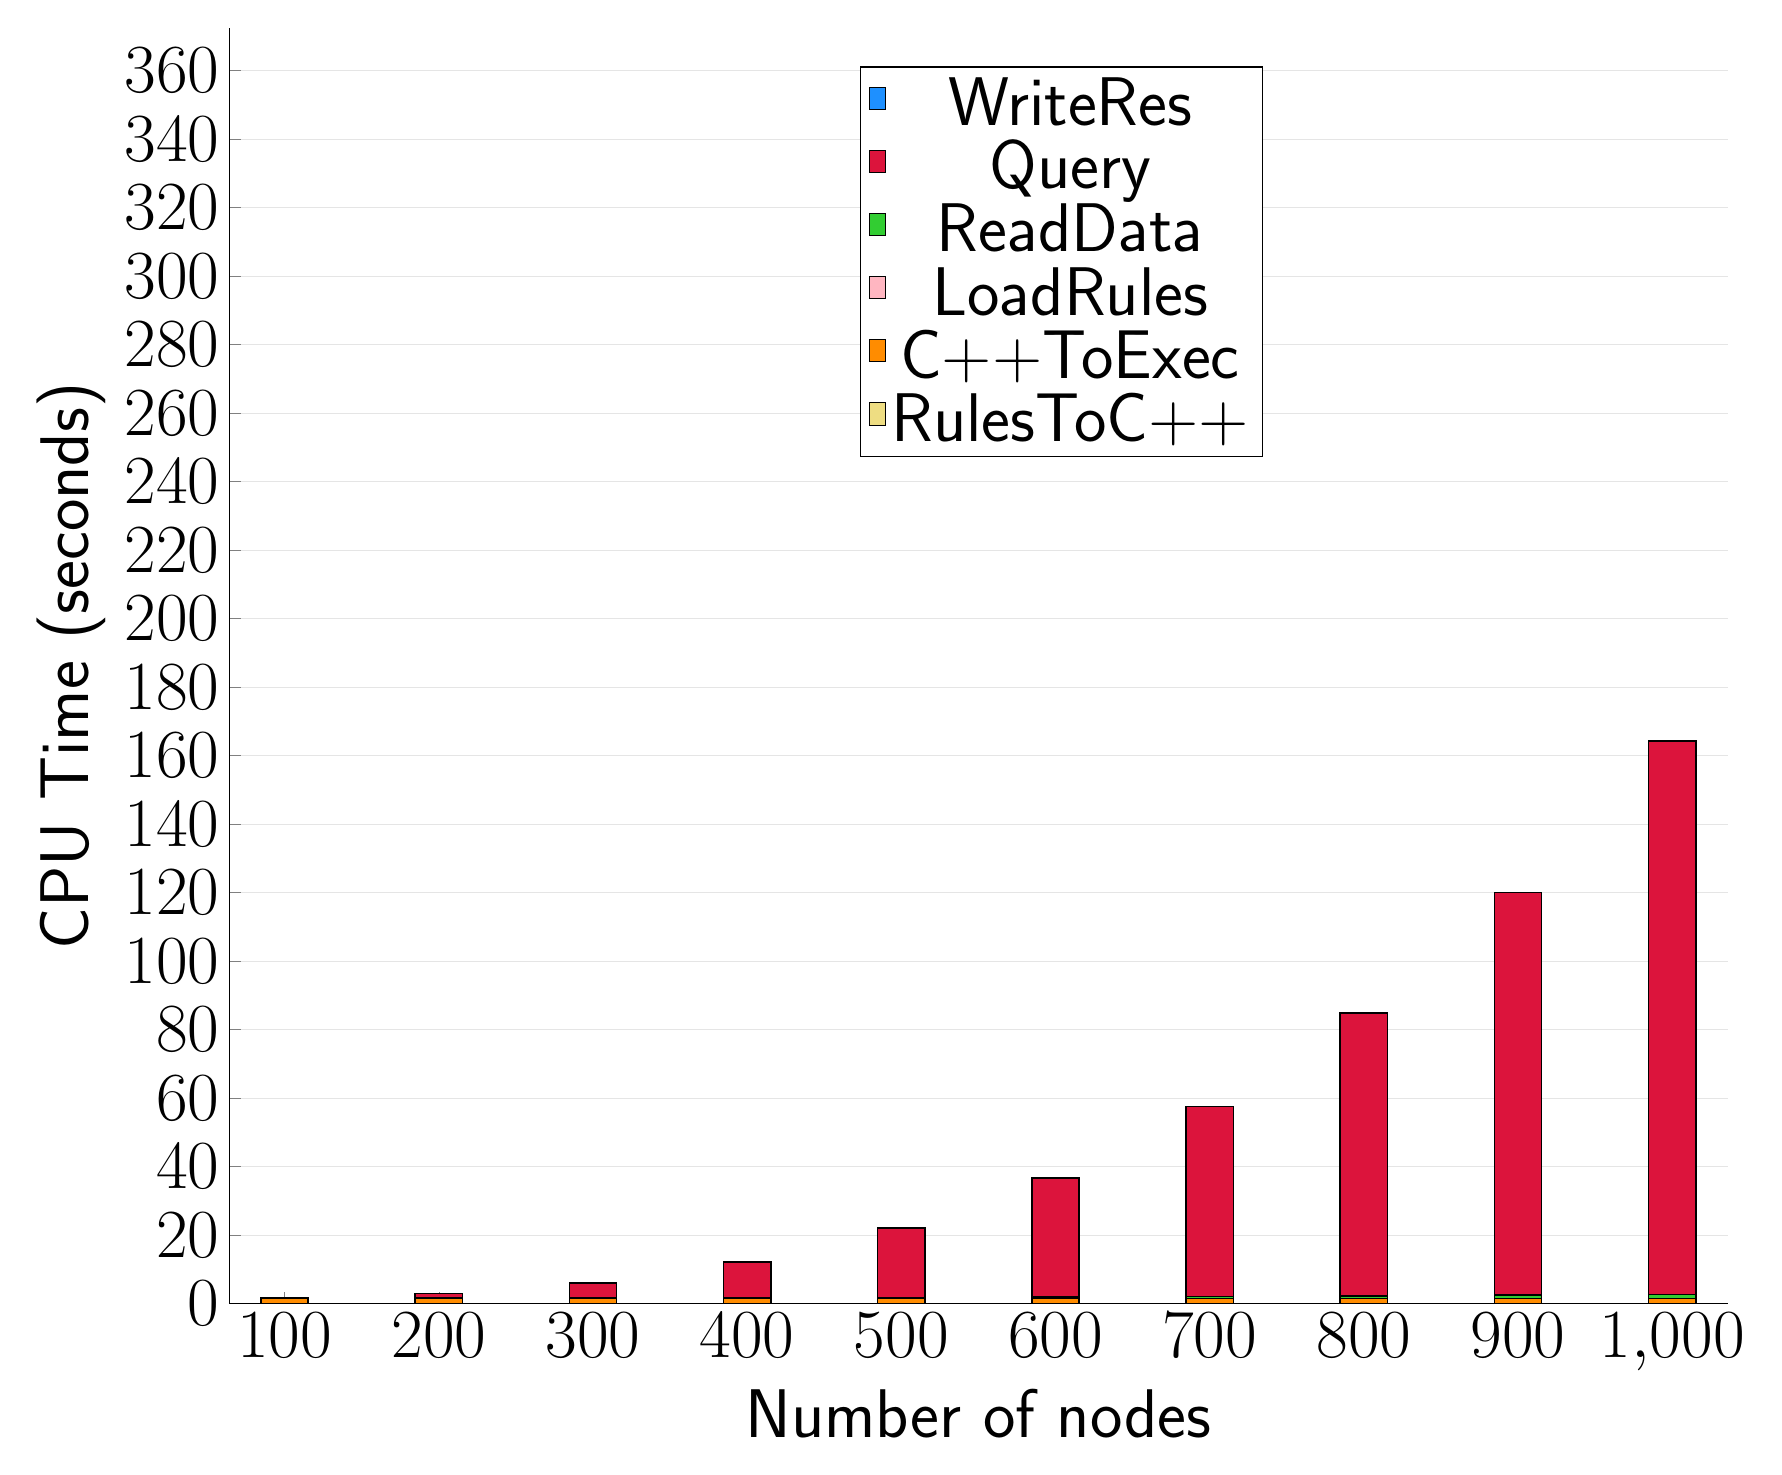
\begin{tikzpicture}
\begin{axis}[
   ybar stacked,
   width=1.7\textwidth,
   bar width=0.6cm,
   ymajorgrids, tick align=inside,
   major grid style={draw=gray!20},
   xtick=data,
   ymin=0, ymax=372.4108,
   axis x line*=bottom,
   axis y line*=left,
   enlarge x limits=0.04,
   legend style={
       at={(0.69, 0.97)},
       anchor=north east,
       legend columns=1,
       font=\Huge,
   },
   ylabel={CPU Time (seconds)},
   xlabel={Number of nodes},
   label style={font=\Huge},
   tick label style={font=\Huge},
]
\addlegendimage{fill=DodgerBlue, draw=black, line width=0.2pt}
\addlegendentry{WriteRes}
\addlegendimage{fill=Crimson, draw=black, line width=0.2pt}
\addlegendentry{Query}
\addlegendimage{fill=LimeGreen, draw=black, line width=0.2pt}
\addlegendentry{ReadData}
\addlegendimage{fill=LightPink, draw=black, line width=0.2pt}
\addlegendentry{LoadRules}
\addlegendimage{fill=DarkOrange, draw=black, line width=0.2pt}
\addlegendentry{C++ToExec}
\addlegendimage{fill=LightGoldenrod, draw=black, line width=0.2pt}
\addlegendentry{RulesToC++}
\addplot +[fill=LightGoldenrod, draw=black, line width=0.55pt] coordinates {
(100, 0.0020000000000000005)
(200, 0.010000000000000002)
(300, 0.010000000000000002)
(400, 0.008000000000000002)
(500, 0.010000000000000002)
(600, 0.0020000000000000005)
(700, 0.0020000000000000005)
(800, 0.0)
(900, 0.0)
(1000, 0.0)
};
\addplot +[fill=DarkOrange, draw=black, line width=0.55pt] coordinates {
(100, 1.566)
(200, 1.5340000000000003)
(300, 1.536)
(400, 1.5340000000000003)
(500, 1.532)
(600, 1.536)
(700, 1.532)
(800, 1.532)
(900, 1.528)
(1000, 1.524)
};
\addplot +[fill=LightPink, draw=black, line width=0.55pt] coordinates {
(100, 0.00015319999999999998)
(200, 0.0001176)
(300, 0.00014379999999999997)
(400, 0.0001458)
(500, 0.0001456)
(600, 0.0001598)
(700, 0.0001632)
(800, 0.00014620000000000003)
(900, 0.000159)
(1000, 0.00016200000000000003)
};
\addplot +[fill=LimeGreen, draw=black, line width=0.55pt] coordinates {
(100, 0.0244322)
(200, 0.0626924)
(300, 0.12474940000000001)
(400, 0.20307139999999996)
(500, 0.3068416)
(600, 0.433943)
(700, 0.5842034)
(800, 0.7582156)
(900, 0.959757)
(1000, 1.1824819999999998)
};
\addplot +[fill=Crimson, draw=black, line width=0.55pt] coordinates {
(100, 0.1759316)
(200, 1.301846)
(300, 4.360934)
(400, 10.353159999999999)
(500, 20.20776)
(600, 34.74972)
(700, 55.39273999999999)
(800, 82.61312000000001)
(900, 117.513)
(1000, 161.5476)
};
\addplot +[fill=DodgerBlue, draw=black, line width=0.55pt] coordinates {
(100, 0.00020920000000000002)
(200, 0.0003704)
(300, 0.0003948)
(400, 0.0003902)
(500, 0.0003412)
(600, 0.000464)
(700, 0.00041919999999999994)
(800, 0.00041799999999999997)
(900, 0.0005034)
(1000, 0.00048579999999999994)
};
\end{axis}
\end{tikzpicture}

\end{document}
